\documentclass[letterpaper,12pt]{article}

\usepackage[top=1in, left=1.25in, right=1.25in, bottom=1in]{geometry}
\usepackage[utf8]{inputenc}
\usepackage[T1]{fontenc}
\usepackage[spanish]{babel}
\usepackage{graphicx}
\usepackage{caption}
\usepackage{float}
\usepackage[backend=biber,style=numeric,sorting=none]{biblatex}
\usepackage{amsmath}
\addbibresource{bib/referencias.bib}

\begin{document}

\tableofcontents
\clearpage

\section{Introducción}

\begin{itemize}
\item \textbf{Planteamiento del Problema:} Se busca implementar una aplicación en Java que permita calcular la distancia entre dos puntos y establecer una correcta comunicación entre distintas clases.  

\item \textbf{Motivación:} En esta práctica lograremos implementar de manera adecuada la comunicación entre clases en archivos por separado, creando dentro de el programa principal diferentes objetos de cada clase para hacer una correcta ejecución con la salida solicitada.

\item \textbf{Objetivos:} Implementar un programa que capture las coordenadas de dos puntos y realizar el cálculo de la distancia entre estos, para finalmente mostrar la distancia obtenida al usuario haciendo uso de una ventana interactiva. 
Comprender y aplicar la creación de objetos y la comunicación entre clases, utilizando objetos como argumentos en los métodos de otras clases.


\end{itemize}
\section{Marco Teórico}

\textbf{Distancia entre dos puntos:} Es la longitud de la línea recta que une a dos puntos. Se calcula aplicando la fórmula: ~\cite{distancia}
\[
d = \sqrt{(x_2 - x_1)^2 + (y_2 - y_1)^2}
\]

\section{Desarrollo}

\textbf{Librerías, clases y paso de mensajes:}

En esta practica utilizamos 2 librerías para la interfaz gráfica de la ventana, así como la librería \textbf{Math}, para el calculo de la distancia entre 2 puntos, que ya viene incluida sin tener que importarla.

Las librerías usadas para la ventana son \textbf{javax.swing.*} y \textbf{java.awt.event.*} (el asterisco significa que se importan todas las clases de ese paquete). \textbf{swing} contiene clases para implementar interfaces gráficas, permite crear ventanas, botones, etiquetas, campos para la entrada de texto, etcetera ; mientras que \textbf{awt.event} contiene clases para manejar eventos, como el manejo de clicks, escritura o cerrar la ventana.

En la clase \textbf{Ventana}, que utiliza estas librerías, declaramos el constructor que recibe dos objetos de tipo \textbf{Punto} y un objeto de tipo \textbf{Mensaje}. Dentro del constructor, se declara el nombre, tamaño, y la forma en la que se cierra la ventana. También un botón y la acción que ocurre al darle click: se crea una cadena que recibe lo que regresa el método \textbf{mensaje} de la clase \textbf{Mensaje} utilizando los valores de los puntos y la distancia entre ellos. 

De esta forma, la clase \textbf{Ventana} se comunica con la clase \textbf{Mensajes}, y esa clase se comunica con la clase \textbf{Punto}. La clase \textbf{Practica4}, donde esta el \textbf{main}, se comunica con todas las clases.

En la clase \textbf{Mensajes}, es en donde se calcula la distancia entre 2 puntos usando el método \textbf{Math.hypot();}, que calcula la hipotenusa de un triangulo rectángulo con base a las diferencias de coordenadas. Esta es la misma formula usada para calcular la distancia entre 2 puntos en un plano. El método \textbf{mensaje} de esta clase, calcula ese valor, y regresa una cadena con los datos de los puntos y la distancia entre ellos.

La clase \textbf{Punto}, en su constructor recibe los valores de sus dos coordenadas, y los referencia a esa clase con \textbf{this}. De esa forma,  los objetos de tipo \textbf{Punto} guardan los valores de cada punto ingresado.

La clase \textbf{Practica4}, en donde esta el main, pide que se ingresen los valores de los puntos desde la ejecución, luego convierte esos valores a double y crea sus respectivos objetos tipo \textbf{Punto}, así como el objeto de tipo \textbf{Mensaje}, para posteriormente crear el objeto de tipo \textbf{Ventana}, pasar los objetos y mostrar el resultado.

Usamos la sobrecarga de métodos en la clase \textbf{Ventana} y \textbf{Punto}, en la primera clase, un constructor no recibe parámetros, y eso muestra una ventana pidiendo ingresar los valores desde la ejecución; el otro constructor recibe los objetos, y esto para mostrar todo lo explicado anteriormente. En la clase \textbf{Punto}, un constructor no recibe parámetros, y el otro si, que es el usado en la práctica.

\section{Resultados}

\begin{figure}[H]
 \centering
    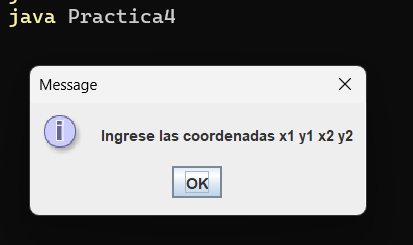
\includegraphics[width=1\textwidth]{Imagenes/p4.png}
    \caption*{Ejecución sin ingresar argumentos}
\end{figure}

\begin{figure}[H]
 \centering
    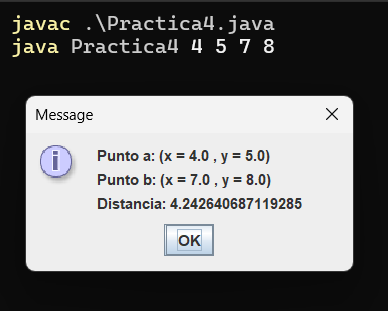
\includegraphics[width=1\textwidth]{Imagenes/ejecucion.png}
    \caption*{Manera correcta de ejecución y salida}
\end{figure}

\section{Conclusiones}
La práctica, además de ayudar como introducción al uso de ventanas emergentes e interfaces gráficas, ayudó bastante al entendimiento de creación de objetos y comunicación entre clases. Se comprendió como utilizar objetos de una clase como argumentos de otra clase, observando a su vez el funcionamiento de la sobrecarga de métodos y su gran utilidad dependiendo del caso. En este caso permitió crear distintos tipos de objeto de tipo \textbf{Ventana} según los valores dados por el usuario.

\printbibliography

\clearpage

\section{Reto para token}

Para la resolución del token, primero buscamos la forma en la que podíamos evaluar si 3 puntos contenidos en un plano cartesiano forman un triangulo equilátero, para eso tomamos en cuenta 2 cosas. La primera fue que la distancia entre cada punto fuera igual, lo que eso significaba que los tres puntos formaban lados del mismo tamaño, usando la misma fórmula que usamos en esta práctica. La segunda fue calcular el área que se forma dentro de esas lineas, si el área era igual a 0, significaba que los puntos formaban lineas colineales y por lo tanto no forman un triangulo equilátero.

La fórmula que utilizamos para calcular el área del triángulo con las coordenadas de sus tres vértices es la siguiente:
\[
A = \frac{1}{2} |x_1(y_2 - y_3) + x_2 (y_3 - y_1) + x_3 (y_1 - y_3)|
\]

Para el cálculo de la distancia, y verificar si eran iguales los lados, usamos \\\textbf{Math.round()} para redondear los valores ingresados, ya que en terminal es inexacto ingresar números irracionales en decimal, y de esa manera nunca van a coincidir los lados, entonces se redondea el resultado.

\begin{figure}[H]
 \centering
    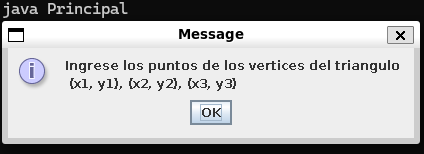
\includegraphics[width=.8\textwidth]{Imagenes/reto1.png}
    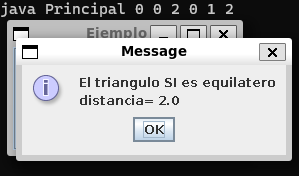
\includegraphics[width=.8\textwidth]{Imagenes/reto2.png}
    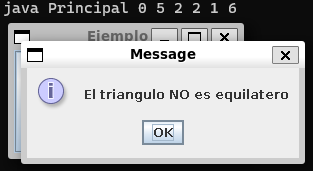
\includegraphics[width=.8\textwidth]{Imagenes/reto3.png}
    \caption*{Ejecución del reto y los posibles resultados}
\end{figure}


\end{document}